%!TEX root = coatli.tex

\chapter{Secondary Focus Mechanism}
\label{chapter:secondary}

\section{Description}

\begin{figure*}
\begin{center}
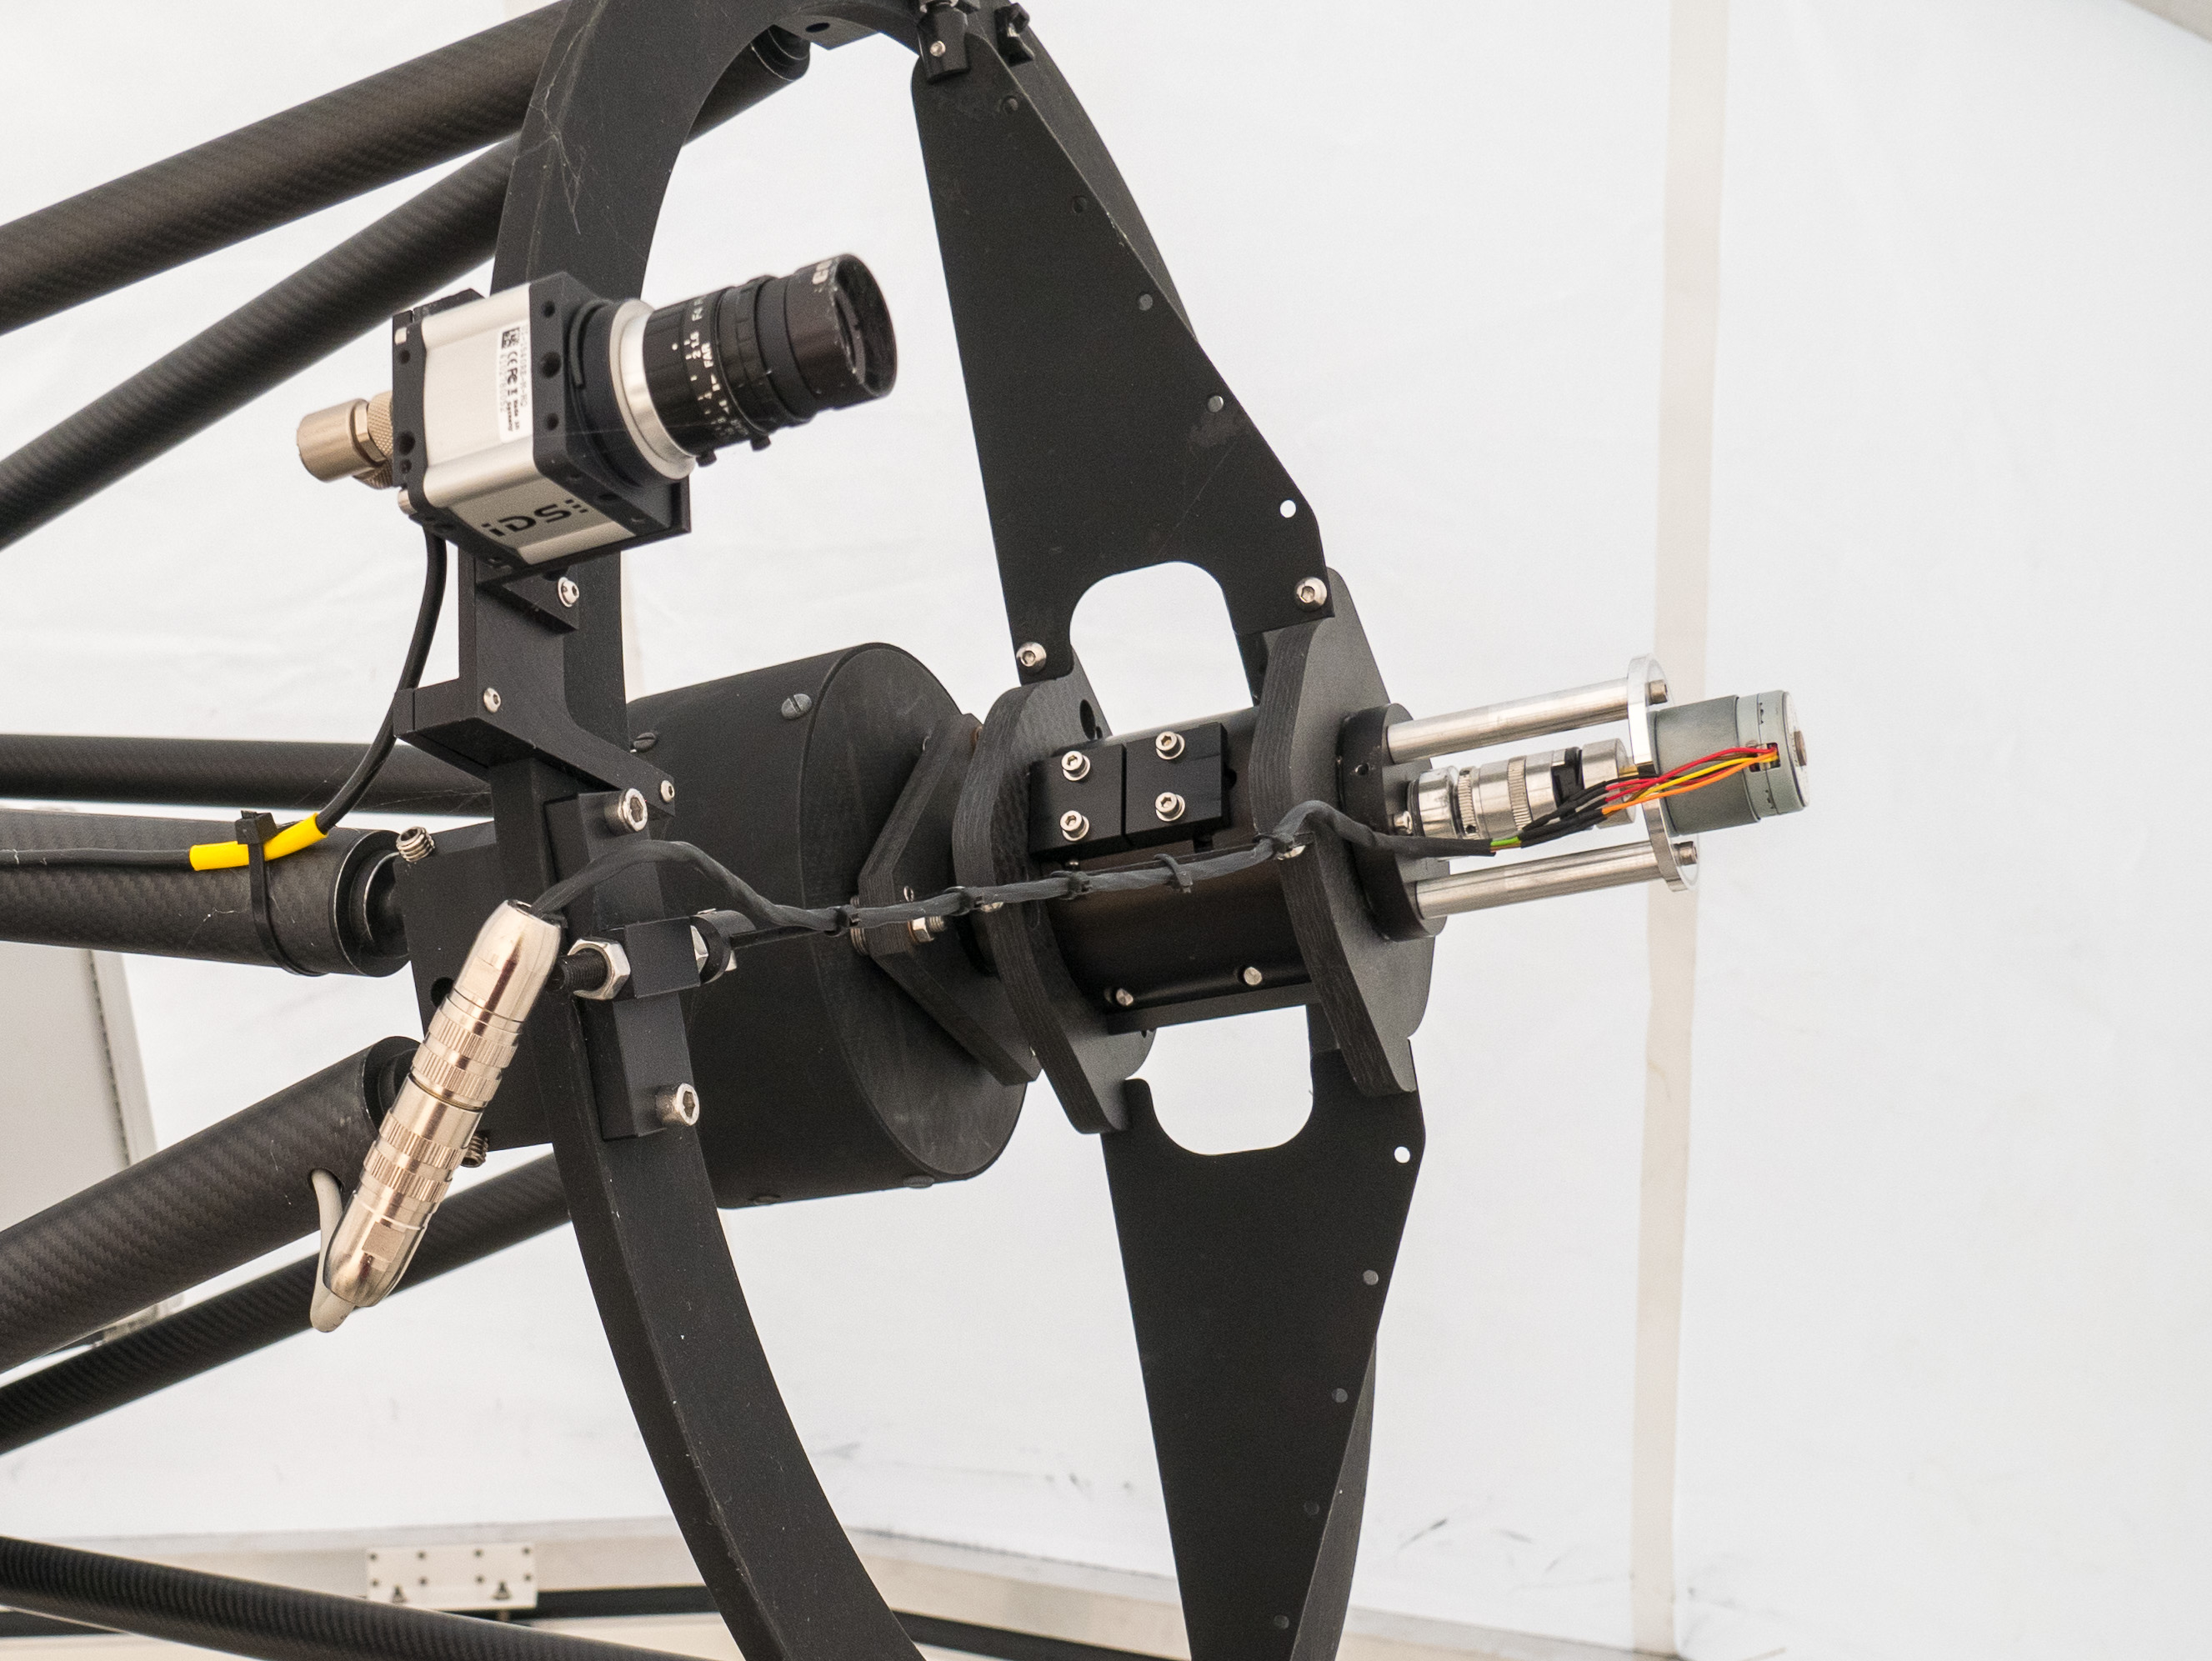
\includegraphics[width=0.7\linewidth]{figures/secondary-coatli-mechanism.jpg}
\caption{The secondary focus mechanism with its cover removed.}
\label{figure:secondary-mechanism}
\end{center}
\end{figure*}

\begin{figure*}
\begin{center}
\begin{labeled}{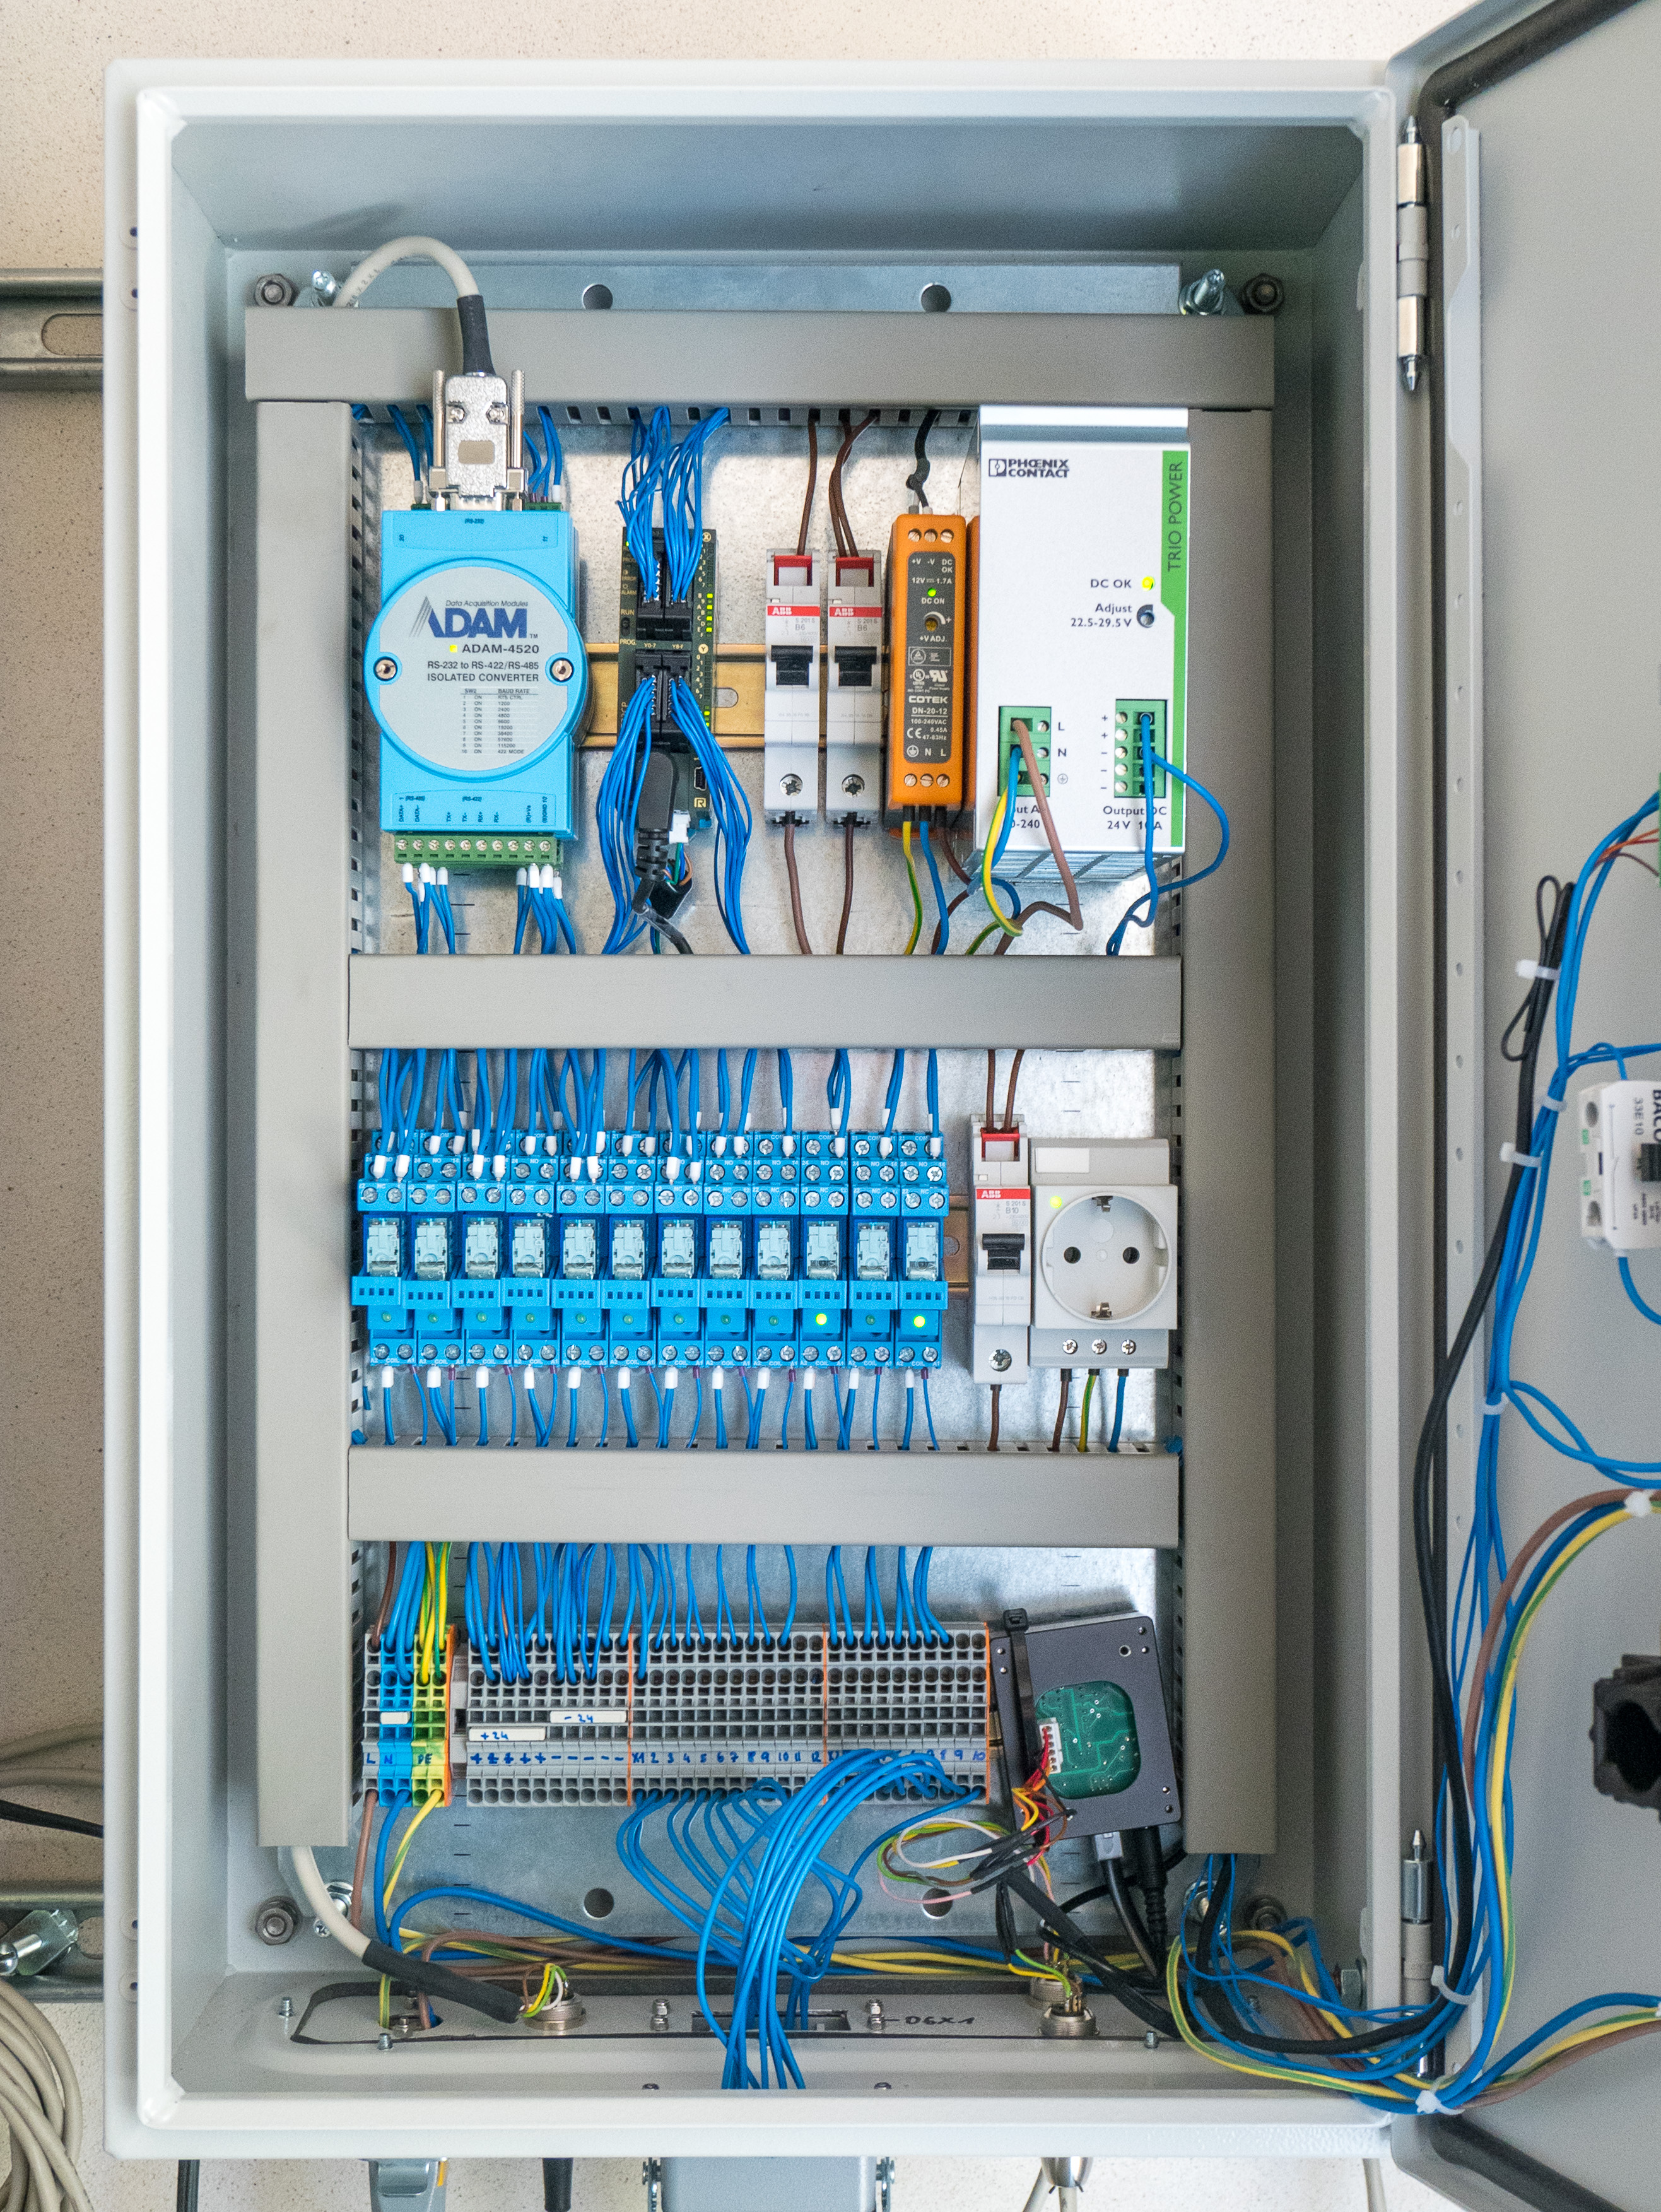
\includegraphics[width=0.6\linewidth]{figures/secondary-coatli-controller.jpg}}
\arrowandlabel{(1.0,-2.4)}{(-0.9,-1.7)}{east}{Controller};
\end{labeled}
\caption{The secondary focus mechanism controller in the covers cabinet.}
\label{figure:secondary-controller}
\end{center}
\end{figure*}

The secondary mirror cell is mounted on a mechanism that allows it to move axially to focus the telescope.

The mechanism, shown in Figure~\ref{figure:secondary-mechanism}, appears to be an adaptation of an Optec TCF-S focuser. 

The controller for the secondary focus mechanism is located in the cabinet of the covers controller in the shed, and is shown in Figure~\ref{figure:secondary-controller}. Communication is via the Lantronix ethernet-to-serial server.

The mechanism does not appear to have an encoder, but rather appears to use a stepper motor and then count steps. The range of 0 to 7000 steps corresponds to 5.6 mm of motion (0.8 {\micron} per step), with 0 corresponding to the secondary at its lowest position (closest to the primary). The absolute calibration appears to be achieved by a combination of moving the motor to 7000 steps when it is powered on and a adjustable block and a hard stop that together define a reference position.

The position of the secondary cell on the focus mechanism can be adjusted manually.

TODO: Block diagram of hardware.

TODO: Control protocol.

\section{Maintenance Procedures}

\subsection{Static Adjustment of the Focus Range}
\label{section:secondary:static-adjustmentl}

This procedure describes how to statically adjust the range over which the secondary can be moved.

\begin{figure*}
\begin{center}
\begin{labeled}{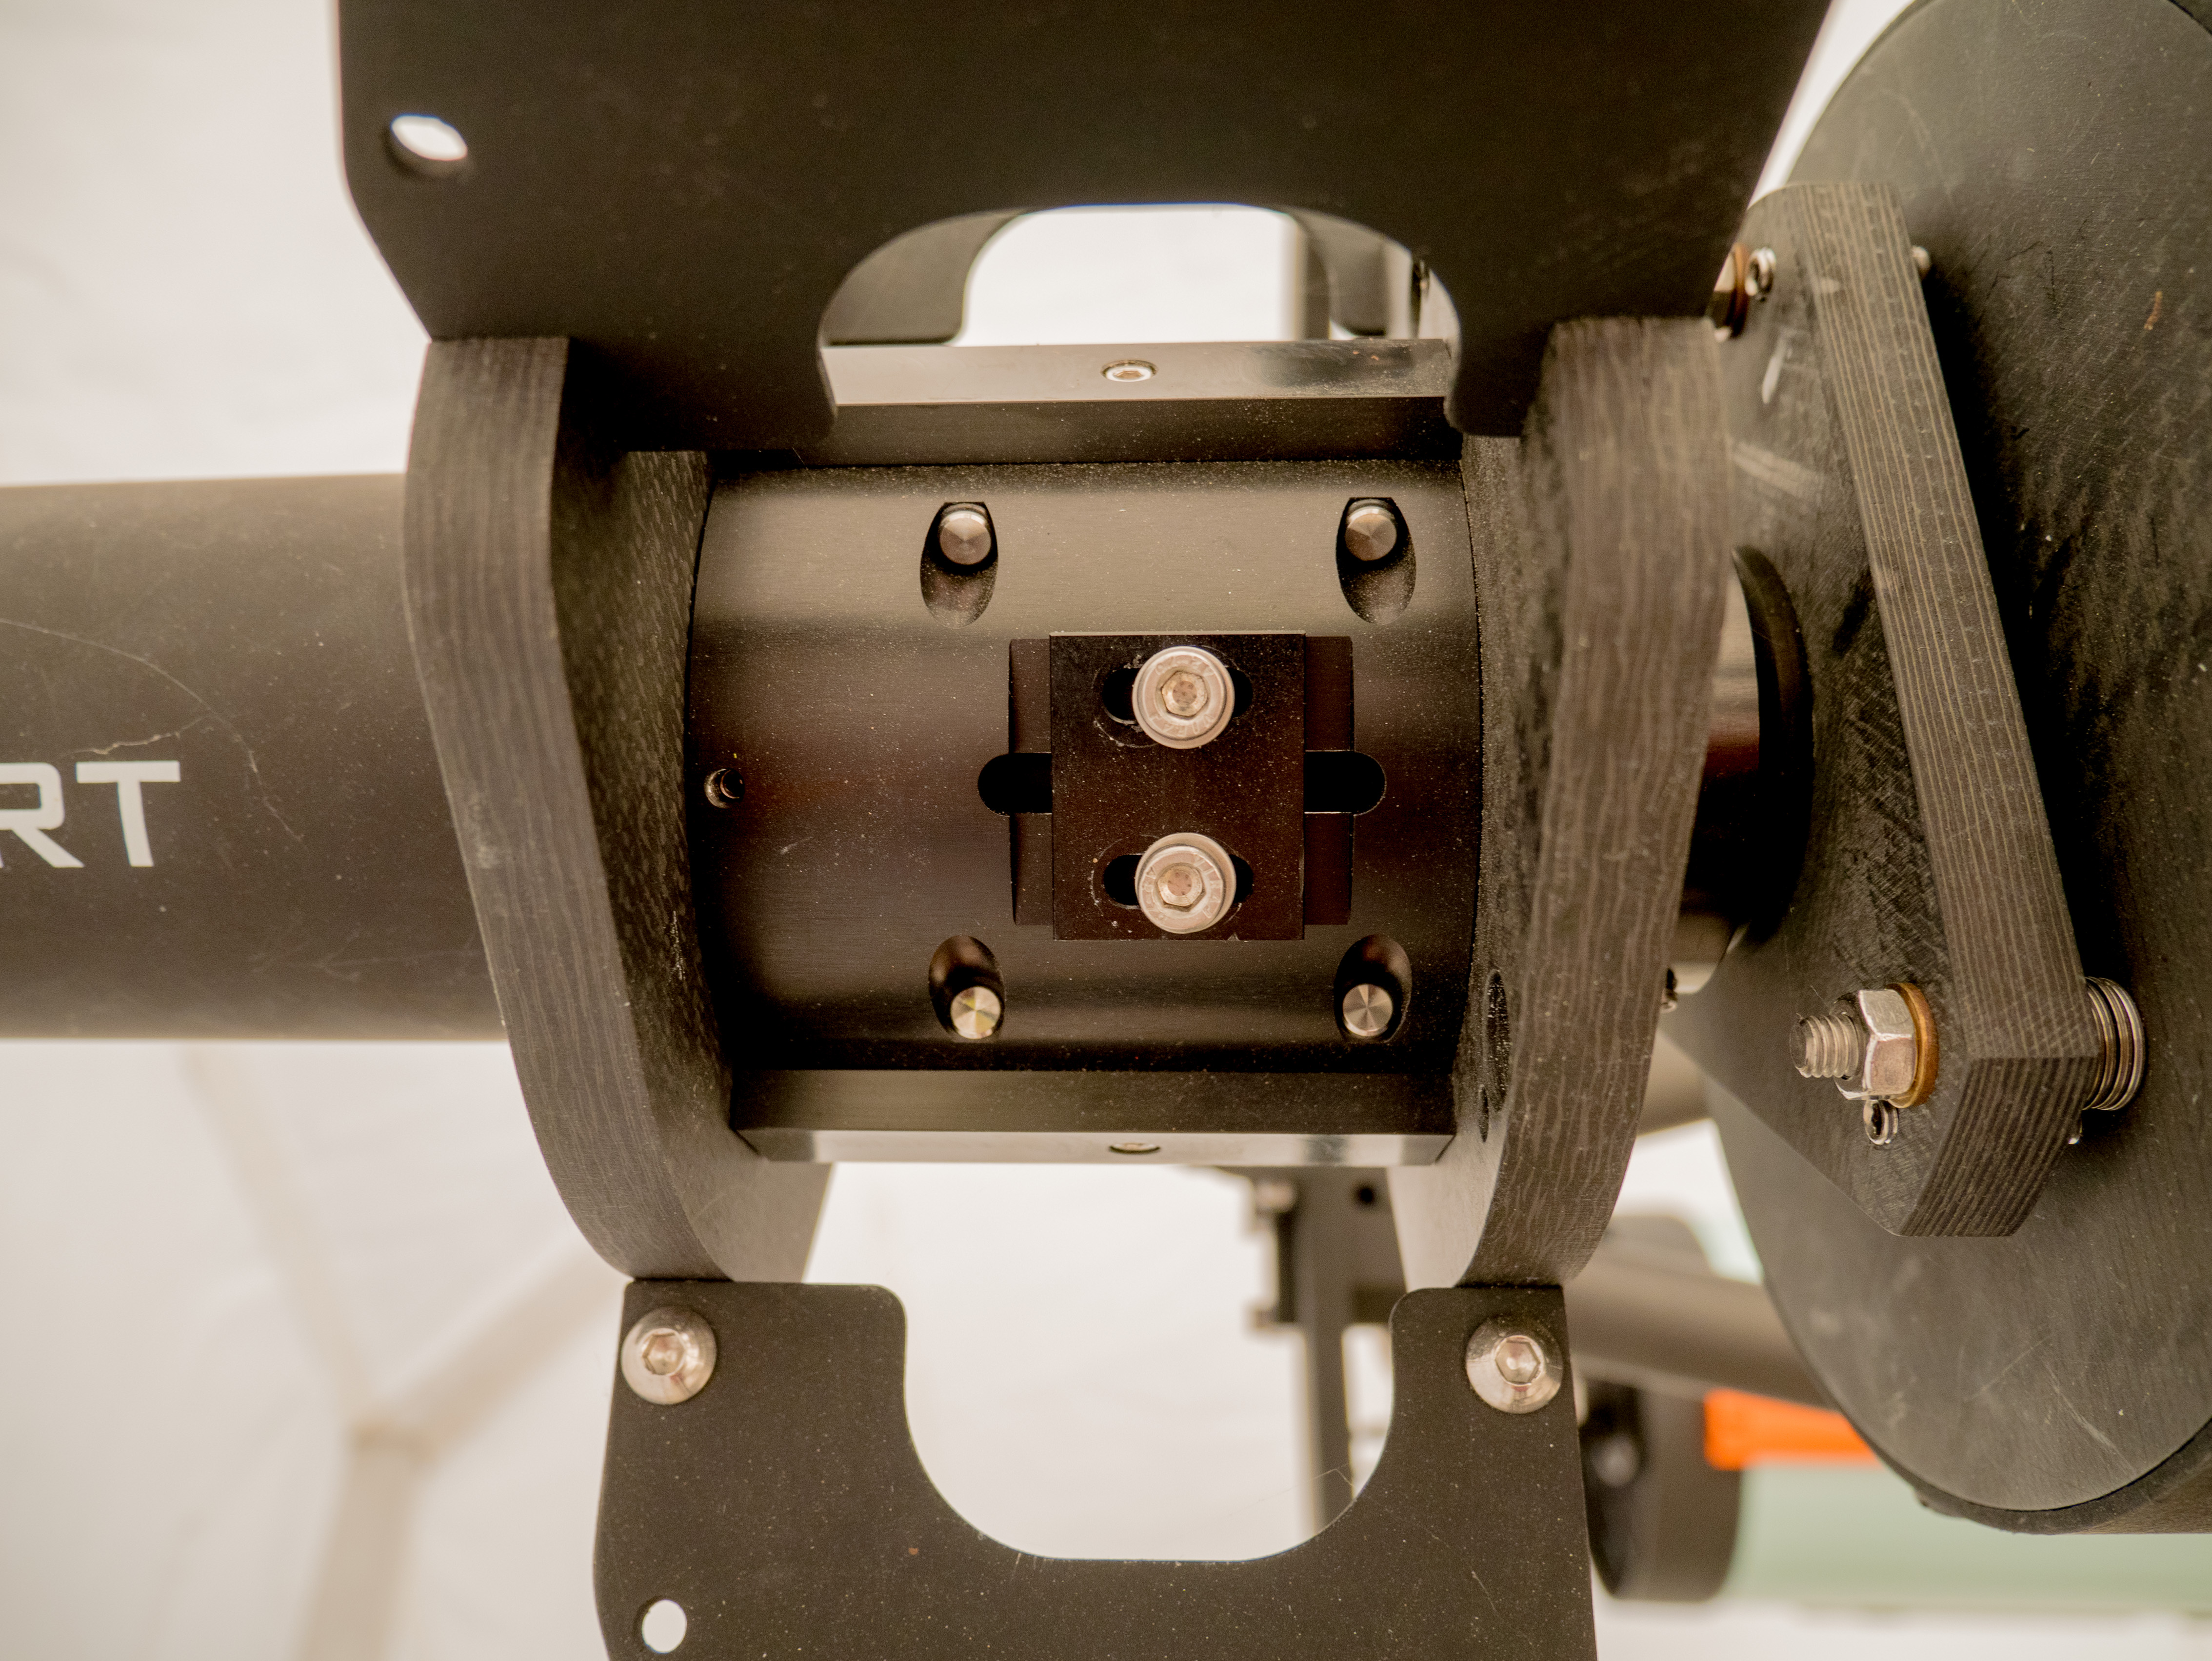
\includegraphics[width=0.8\linewidth]{figures/secondary-coatli-adjustment.jpg}}
\arrowandlabel{(-0.4,-0.0)}{(-3.0,-2.2)}{east}{Hard Stop};
\arrowandlabel{(0.3,0.2)}{(3.0,-2.2)}{west}{Block};
\end{labeled}
\caption{The secondary focus mechanism adjustment. When the secondary focus mechanism is switched on, the mechanism moves upwards until the block comes into contact with the hard stop. This defines position 7000. The mechanism then moves back to 3400.}
\label{figure:secondary-adjustment}
\end{center}
\end{figure*}

\subsubsection{Safety Considerations}

\safety{Use a harness, line, and helmet when you work on the platform or balconies.}

\subsubsection{Requirements}

You will need:
\begin{itemize}
\item At least two persons.
\item The key to the shed (see \S\ref{section:shed-key}).
\item Metric hex keys. TODO: Size
\end{itemize}

\subsubsection{Procedure}

TODO: Photo.

\begin{enumerate}
\item Turn off power to the secondary controller, either by switching off power to the covers cabinet manually or by running
\begin{quote}
\verb|tcs request power switchoff secondary|
\end{quote}
\item Adjust the position of the block. When the secondary focus mechanism is switched on, the mechanism moves upwards until the block comes into contact with the hard stop. This defines position 7000. The mechanism then moves back to 3400. See Figure~\ref{figure:secondary-adjustment}.
\item Turn on the power to the secondary controller, either by switching on the covers cabinet manually or by running 
\begin{quote}
\verb|tcs request power switchon secondary|
\end{quote}
\end{enumerate}

\section{Remote Interface}

\subsection{Lantronix EDS}
\label{section:secondary-lantronix-eds}

The RS-232 interface to the secondary controller is made available via the Lantronix EDS 4100 ethernet-to-serial converter. Specifically, it is connected to line 2 and configured as 19200/8-N-1 with a tunnel on TCP port 10002.

The Lantronix EDS is on the LAN at \verb|serial|.

\section{Control}

The server for the secondary runs on \verb|control|. 

The server starts automatically after \verb|control| is boots, but if necessary can be stopped, started, or restarted explicitly by issuing the following shell commands on \verb|control|:
\begin{itemize}
\item
\verb|sudo stopserver secondary|
\item
\verb|sudo startserver secondary|
\item
\verb|sudo restartserver secondary|
\end{itemize}

Server requests can be issued from any of the Mac or Linux machines on the LAN. The following requests are supported:

\begin{itemize}
\item
\verb|request secondary initialize|

Initialize the server and secondary hardware. As part of the process of initializing, the secondary will more to its initial position.

For this request to be accepted, the server activity must not be \verb|starting| or \verb|error|.

If the request is accepted, the server activity changes to \verb|initializing| and then, once it has initialized, to \verb|idle|.

\item
\verb|request secondary move| \var{z0}

Move the secondary to position \var{z0}.

For this request to be accepted, the server activity must not be \verb|starting|, \verb|started|, \verb|initializing|, or \verb|error|.

If the request is accepted, the server activity changes to \verb|moving| and then, once it has opened to the specified angle, to \verb|idle|.

The nominal position \var{z0} is converted to a raw position by applying corrections for the filter, position, and temperature.

\item
\verb|request secondary stop|

Stop the secondary.

For this request to be accepted, the server activity must not be \verb|starting| or \verb|error|.

If the request is accepted, the server activity changes to \verb|stopping| and then, once it has stopped, to \verb|started| (if the server has not been initialized) or to the activity after the previous completed request.

\item
\verb|request secondary reset|

Reset an error in the secondary.


\item
\verb|request secondary status|

Show the status of the server.

Obtain the values of the status data from the server and print them to stdout.
\end{itemize}

\section{Bibliography}

\begin{flushleft}
\begin{itemize}
\item “\href{bibliography/secondary-coatli/tcs-f-manual.pdf}{TCS-F Technical Manual}”, Optec Inc, Revision 11, August 2010.
\end{itemize}
\end{flushleft}